\chapter{Application Release}
\label{ch:testing}

Before application can be released to production it should be properly tested. In this last chapter, the development process is outlined, automated unit testing and pull-request approach of development even as single developer. Later on, the process of incrementally tested application though internal a beta testing channels on the Android devices is explained. In the end, released version of the application is shown along with link to \textit{Google Play Store}. 

\section{Development Workflow}
Coffee Time was developed as fully open-sourced (MIT licensed) application available at GitHub. Even as a single developer, author wanted to have full control over development process. The development workflow was setup accordingly:

\begin{itemize}
    \item \textit{Master} branch is production code. Code within \textit{master} has to be fully tested, working code. Each commit within \textit{master} branch has to have own tag -- version number.
    \item \textit{Dev} branch is for active development. 
    \item Each feature or bug has assigned GitHub \textit{issue}.  
    \item Each feature is developed within its own \textit{feature} branch, branched from \textit{dev} branch. The~\textit{feature} branch has to be named as \verb|feature/X| where X is the~issue number.
    \item Each bug has its own \textit{fix} branch and is named as \verb|fix/X| where X is an~issue number.
    \item Every feature and bug fix has to be merged to \textit{dev} branch through GitHub \textit{Pull Request}.
    \item Each \textit{Pull Request} can be completed only if automated build with unit tests is successful.
    \item Each commit contains reference to an~issue number. 
\end{itemize}

Moreover, created issues has assigned \textit{labels}, such as architecture, design or bug, for higher clarity and each issue is assigned to the milestone. This helped to organize remaining work and stick to the plan. 

% For some reason, it still prints within \begine{itemize} -- this works...
\begin{listing}[ht]
\begin{minted}{yaml}
name: 'Mobile - Build and test'
on:
   push:
      paths: mobile/**
      branches: [feature/**, fix/**, dev]
jobs:
   build-and-test: 
    runs-on: ubuntu-latest
    steps:
    - uses: actions/checkout@v1 
    - uses: actions/setup-java@v1
      with:
        java-version: '12.x'
    - uses: subosito/flutter-action@v1
      with:
         channel: 'stable'
    # Get flutter packages
    - name: 'pub get'
      working-directory: mobile
      run: flutter pub get
   # Build runner
    - name: 'pub runner'
      working-directory: mobile
      run: flutter pub run build_runner \ 
           build --delete-conflicting-outputs
    # Build
    - name: 'build'
      working-directory: mobile
      run: flutter build aot
    - name: 'test'
      if: always() && !cancelled()
      working-directory: mobile
      run: flutter test
\end{minted}
\caption{Configured GitHub Action.}
\label{listing:gh-ci}
\end{listing}

\subsection{Continuous Integration}

GitHub has a feature called GitHub Actions -- automation of the development workflow. Whenever pull request is created or new commits are pushed to created pull requests or \textit{dev} branch, an automated action is run. This action checkouts current code, build it with Flutter tools and run unit tests. If any of those action fails, build is marked as failed and in case of a pull request, pull request can not be closed. 

Configuration of GitHub Actions are done through configuration files within YAML format. Coffee Time build action configuration is shown in~\Cref{listing:gh-ci}. Action is triggered on push to \textit{feature}, \textit{fix} or \textit{dev} branch and only if change set contains any file within \textit{mobile} folder. Java and Flutter tools are installed in order to build Flutter application. Before building application, Dart packages has to be downloaded. Finally after the application is built, unit tests are started. If any of tests failed, whole action is marked as failed.

\section{Internal Testing}
In the moment, when application had minimal working feature, internal testing channel on \textit{Google Play Services} was created in order to have early feedback from internal testers. Internal Channel provides access to applications in early stages to selected users. In case of Coffee Time application, internal testers were author's closest persons and family members. A~number of testers were up to ten people and during development, they gave valuable feedback. An~example of such feedback was not working navigation action on some Android versions. 

During development, several versions were published for internal testing:

\begin{itemize}
    \item \textbf{v0.0.1} -- First internal test flight. Implemented nearby search without filter functionality. Other features were not available. 
    \item \textbf{v0.1.0} -- Added filter functionality, multi language support, fixed several bugs. Design improvement. 
    \item \textbf{v0.2.0} -- Added map functionality. Fixed several issues with API communication. Filtering changes and bug fixes.
    \item \textbf{v0.2.1} -- Hotfix version. Fixed bug when application crashed in case of GPS was turned off. 
    \item \textbf{v0.3.0} -- Performance and stability fixes. 
\end{itemize}

After internal testing, application was opened up for beta testers within \textit{Beta Channel} with version \textit{v0.3.0}. With that version more users tried application and gave more feedback. Based on the feedback, more bugs were fixed and last beta version \textit{v0.3.1} were deployed for test. 

All versions were merged to \textit{master} branch and properly tagged, so each version can be found on GitHub project. 

\section{Crashlytics}
When the application was ready to release another \textit{Firebase} service was added to the~application -- \textit{Crashlytics}~\cite{firebase-crashlytics}. \textit{Crashlytics} is a realtime crash reporter that helps track, prioritize and fix stability issues. The official plugin for \textit{Crashlytics} was used to enable this service. In the application only a~two lines of code had to be added to enable reporting~(\Cref{listing:ct-crashlytics-enable}).

\begin{listing}[h!]
\begin{minted}{dart}
// ... within main() method
Crashlytics.instance.enableInDevMode = kDebugMode;
// pass all uncaught errors from the framework to Crashlytics.
FlutterError.onError = Crashlytics.instance.recordFlutterError;
\end{minted}
\caption{Enable Crashlytics.}
\label{listing:ct-crashlytics-enable}
\end{listing}

\section{User Testing Re-Evaluation}
When the release candidate version was prepared, same user testing as was done with the prototype version was evaluated. Five users were involved in this tests. User profiles varied from their overall mobile application skills to their personal preferences over cafes. 

Test was evaluated in the same manner as before, with same test cases to know, if found issues within prototype were fixed or not. To remind, found issues were:

\begin{questions}
  \item Filter screen is confusing. Confirmation is useless.
         \begin{answer}
          Confirmation within filter screen was removed. When an~user press a~back button, selected filters are applied.
         \end{answer}
    \item Do not open filter screen, just open some modal window to selects tags.
         \begin{answer}
          Filter screen remained the~same as a~more feasible solution by author opinion.
         \end{answer}
    \item The filter icon is unclear.
         \begin{answer}
          Icon remained the same as it is standard icon used across different applications. However, two new testers confirmed once again this confusion. 
         \end{answer}
    \item If an~user is located on the~detail screen, clicking on a~tag icon should set filter.
         \begin{answer}
         For now not implemented. 
         \end{answer}
   \item Three different icons are used to start navigation. Icon is different on the cafe list from icon within detail screen.
         \begin{answer}
          Icons were consolidated into one icon.
         \end{answer}
   \item Cafe's name on tile can be hard to read with the~contrasting background image.
         \begin{answer}
          Solved with darker photo overlay.
         \end{answer}
   \item Landscape mode is not working.
         \begin{answer}
          Landscape mode was disabled. 
         \end{answer}
   \item The map marker could contain more information than the cafe's name only.
         \begin{answer}
          Currently it is not doable due to a~limitation of the maps plugin.
         \end{answer}
\end{questions}

New testers encountered old issue only with ``unclear filter icon''. The~more serious issue was found within the tag review screen. On some screen resolutions, a confirm button to submit review can be ``hidden'' and the user has to scroll down a little bit to see a button. One user was confused as it looked like no button is not visible and pressed back button to confirm review. Such action did not submit review and test case failed. A~solution to prevent this issue could be to use \verb|FloatingActionButton| which is still visible on the~screen. Same approach is used for ``favorite'' button within detail screen.

As the test results did not find any serious issues which could prevent release the application, final steps were taken to deploy the application to the~production.

\section{Release}
Coffee Time was released as version \textit{1.0.0} to the \textit{Google Play Store} for Android devices. In order to publish a release, a proper name and description in all available languages had to be filled before the application could be accepted. Moreover, the store displays application photo, logo and a~cover image. These fields were necessary to fill as well. After the~release, two minor versions \textit{1.0.1} and \textit{1.0.2} were released as hotfixes to prevent application crashes on some devices.

\Cref{fig:ct-released-version} shows released version. In contrast with prototype version (\Cref{fig:hifi}), there are no significant graphical changes other than 

\begin{itemize}
    \item changed font typeface,
    \item moved favourite button from header to FloatingActionButton,
    \item slightly different color pallete.
\end{itemize}

\begin{figure}[h!]
    \centering
    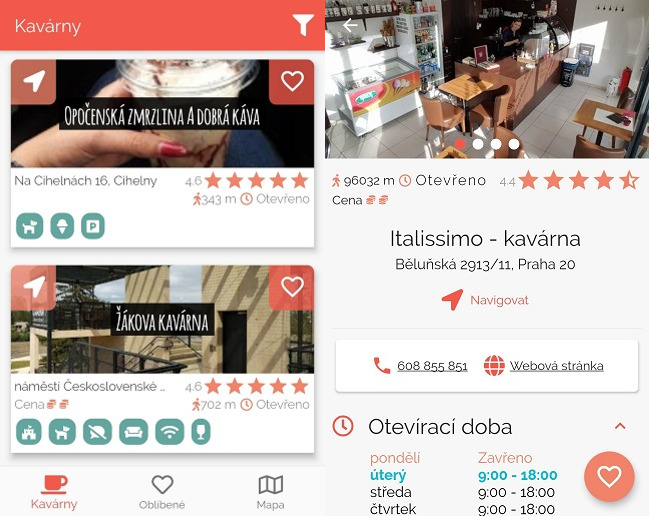
\includegraphics[width=\textwidth]{img/deploy/app.jpg}
    \caption{Released Version -- Cafe List and Detail Screens.}
    \label{fig:ct-released-version}
\end{figure}

\begin{figure}[h!]
    \centering
    
\includegraphics[width=0.33\linewidth]{img/deploy/app-qr.pdf}
    \caption{Coffee Time QR Code for Downloading the Application.}
    \label{fig:ct-qr-code}
\end{figure}

\subsection{Missing Feature from Prototype}
One feature from prototype did not make it to first released version and that is custom search location. In the current version, custom location can be set through map view but not from cafe list. The implementation with this feature is partially done, as the API back-end already partially support it and in the application, the data layer has already methods for that feature.  
However, during implementation was acknowledged that fully functional text search should include autocomplete services from Google Places API. Unfortunately, the current design of API and application did not count with such requirements. Feedback from users includes also a requirement for such features. Thus this feature is considered as the most wanted feature in future development. 

\subsection{Conclusion}
Coffee Time was successful implemented and released to production for \textit{Android} devices. A~\textit{QR} code for downloading is displayed in~\Cref{fig:ct-qr-code}. As Flutter is multi-platform, \textit{iOS} could be deployed too. However there were a~few ``obstacles'' that prevented to do that:

\begin{itemize}
    \item Application design was inspired from Material Design and this design do not correspond with Apple Deisgn,
    \item \textit{iOS} development requires \textit{MacOS} device in order to build \textit{iOS} application,
    \item and finally, goal was to provide fully functional application at least for \textit{Android}. In the future development, the \textit{iOS} version is planned as well. 
\end{itemize}